% \section{Implementation and case studies}
\section{Case study: scheduling in a mobile WSN}
\label{sec:case}

% Case studies motivation:
The power management mechanism described in Section~\ref{sec:epospm} incorporates the proposed heuristics.
% Intro to the ADHOP experiment
Although having a real implementation of the system, the evaluation of the heuristics uses simulation.
This is because of the nature of the studied system, which includes yearlong analysis of system behavior to verify the efficiency of the energy schedulers.
The simulation presented in this paper is that of a dense, mobile network.
This application builds a critical scenario for communication and energy consumption due to the large amount of data exchanged in the network.
The simulation parameters receive data collected from real measurements performed on \emote~nodes powered by rechargeable batteries and solar panels.

The application is a WSN running the Ant-based Dynamic Hop Optimization Protocol (\adhop)~\cite{Okazaki:SCPA:2011} over an IP network using IEEE 802.15.4.
\adhop~is a self-configuring, reactive routing protocol.
The reactive component of \adhop~uses an \emph{Ant Colony Optimization} algorithm to discover and maintain routes.
Ants go out to track routes, leaving a trail of pheromone on their way back.
The selected routes for data exchange are the ones with a higher pheromone deposit.

% Describe ADHOP modification - task table
With the purpose of evaluating the energy scheduling heuristics presented in this paper, we modified \adhop~in order to make it energy-aware.
The tasks implementing \adhop~are now either hard real-time or best-effort, as described in the application model (Section~\ref{sec:app_model}).
The main idea behind this setup is to homogenize the battery discharge for every node in the network to enhance the lifetime of the network as a whole.
Considering the radio as the most energy-hungry component in a wireless sensing node, we toke the design decision of modeling the routing activity of \adhop~as a best-effort task, as shown by the task set at Table~\ref{tab:adhop-taskset}.
The basic node functionalities of sensing a value (task $Sense$) and sending it through the radio to a sink node (task $Send$) where modeled as hard real-time tasks.
Two best-effort tasks implement the functionality of forwarding packets (and ants) coming from other nodes when acting as a ``router'': one monitors the channel for arriving messages ($LPL$ - Low Power Listen) and another receives messages and route them to another node ($Route$).
This approach will cause links to go down when a node realizes it must stop best-effort tasks.
However, ADHOP is a suitable candidate for these modifications because the ACO routing mechanism tries to find alternative routes if a link fails.

\mytabwnote{adhop-taskset}{Parameters for the tasks of the \adhop~case-study.}

% Describe application characteristics (lifetime, battery size, etc)
We fixed the lifetime objective for this system at 30 days.
This means that, all along the system execution, if the energy harvesting mechanism fails, the system will still be able to run its hard real-time tasks for, at least, 30 days.
It is possible to analyze the task set and compute the total energy consumption of the hard real-time tasks to be around $722~mAh$ during the desired lifetime.
Thus, the initial battery charge for the system has to be greater than that to allow the system to reserve energy for the critical part of the application.


% Describe the 2 steps simulation
The evaluation procedure comprises two simulation steps.
% * OmNET++ used to characterize application behavior for different BET rates
In the first step, a simulation using the \textsc{OmNET++} Simulator characterized response of the application to variations in the execution rate of best-effort tasks~(BET rate).
% * Show and discuss first step results
As can be seen in Figure~\ref{figtwo:adhop-char-ddradhop-char-energy}, lower energy consumption at lower BET rates comes at the cost of lower data delivery rate.
% Also, it is possible to observe in the graphic that BET rates above $50\%$ have no significant impact on packet delivery.
% Thus, it is assumed that BET rate will only be adjusted within the range $[0,50]$ as a means to further save energy.

\figtwo
{adhop-char-ddr}{Data delivery per BET rate.}{width=\columnwidth}
{adhop-char-energy}{Avg. power and energy cons. per BET rate}{width=\columnwidth}
{Network response to BET rate.}{0.5\textwidth}


% * After that, energy consumption was simulated for desired lifetime
The second step applies the proposed heuristics to analyze the energy consumption over one year.
Besides the proposed heuristics, the simulations cover two other situations.
In the first one, the scheduler does not impose any constraint on the BET rate.
Although this showed a large gain in the BET rate, it also caused real-time tasks to fail due to the lack of energy.
It shows that the system needs to control energy allocation to handle hard real-time applications.
The second one is a reserve-based approach explored in previous experiments~\cite{Hoeller:SMC:2011}.
In this approach, BET rate is either $100\%$ or $0\%$, depending on the system energy status.
Although this second approach respects the deadline of hard real-time tasks, its wide variation range brings an undesirable instability to the BET rate.

% \mywtab{sim-params}{Simulation parameters.}

Each one of the heuristics proposed here had its parameters set to the best scenario for its execution.
For BGR, the system uses a smaller battery once it shows no large dependency on energy buffer size.
For BWR, however, the system needs a large battery buffer to assure a reasonable BET rate.
That would be a problem if space or weight become an issue for this system as, for instance, 12 AA-size batteries would be needed to provide a system with 12,600~mAh at 3~V.
BWAR and BWDR, although also dependent on the energy buffer size, do not demand extremely large buffers to exist once, with the assumption of incoming energy from the energy-harvesting mechanism, they are able to compensate for the low share of stored energy they use.

% * Show and discuss final results
% \mywtab{sim-results-taskset}{Simulated taskset results.}

\figtwo
{plot_1year}{1998 monthly irradiation.}{width=\columnwidth}
{bet_rate_1m}{BET rate during 1998.}{width=\columnwidth}
{BET rate variations over the 1-year simulation.}{.5\textwidth}

\begin{figure}[ht]
	\centering
	\begin{subfigure}[b]{.5\textwidth}
		\centering
		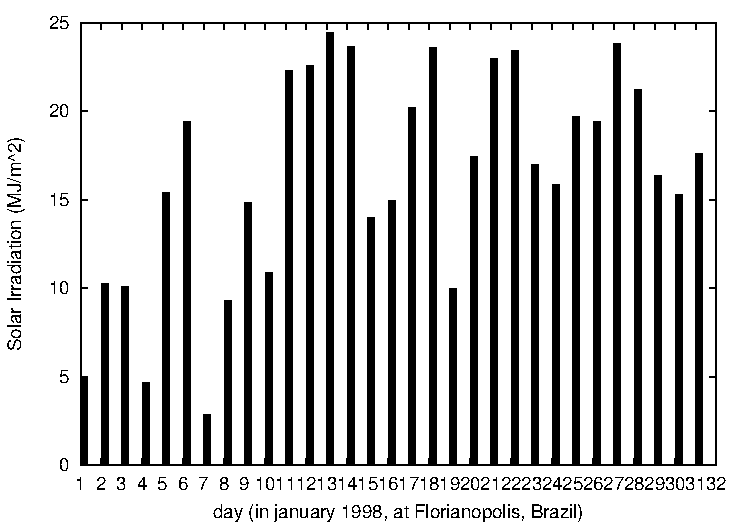
\includegraphics[width=\columnwidth]{fig/plot_daily_jan}
		\caption{January 1998 daily irradiation.}
	\end{subfigure}%
	\begin{subfigure}[b]{0.5\textwidth}
		\centering
		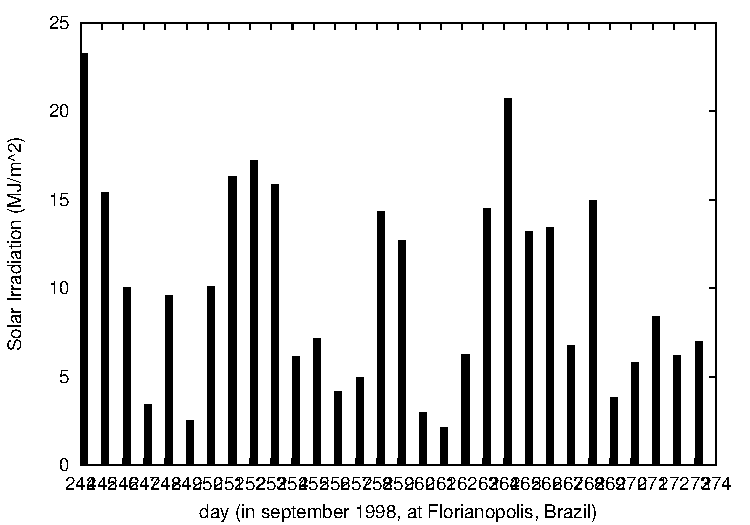
\includegraphics[width=\columnwidth]{fig/plot_daily_sep}
		\caption{September 1998 daily irradiation.}
	\end{subfigure}%
	
	\begin{subfigure}[b]{0.5\textwidth}
		\centering
		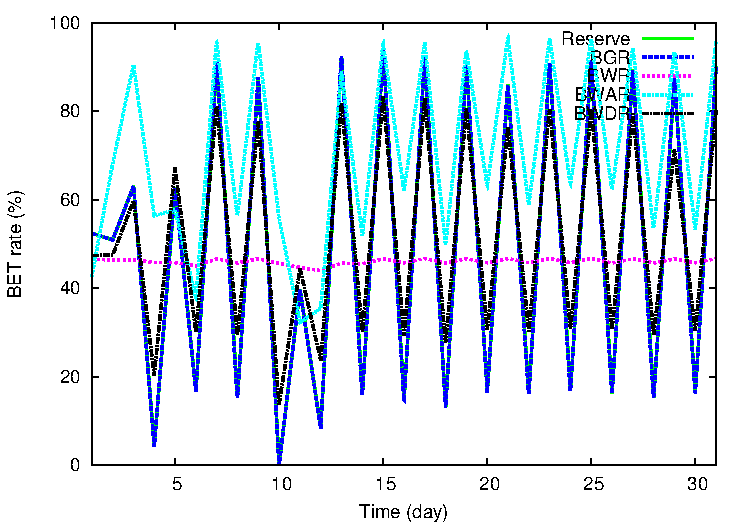
\includegraphics[width=\columnwidth]{fig/bet_rate_1d_jan}
		\caption{BET rate during January 1998.}
	\end{subfigure}%
	\begin{subfigure}[b]{0.5\textwidth}
		\centering
		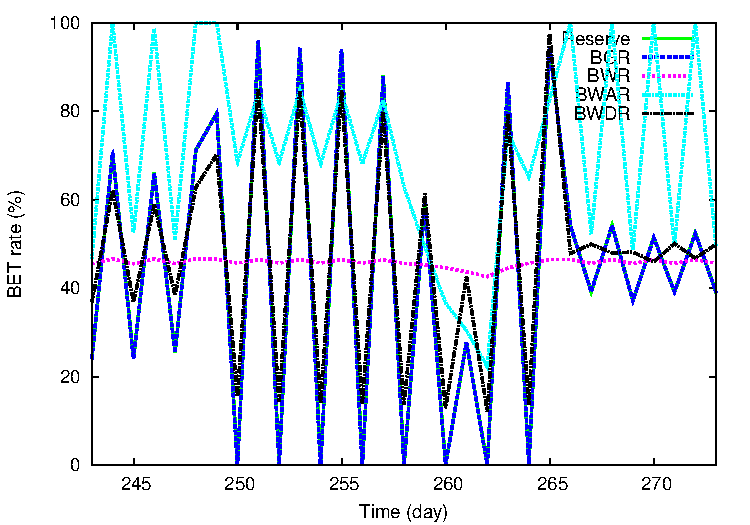
\includegraphics[width=\columnwidth]{fig/bet_rate_1d_sep}
		\caption{BET rate during September 1998.}
	\end{subfigure}

    \caption{BET rate variations over a summer and a winter months.\label{figfour:1}}
\end{figure}


\begin{figure}[ht]
	\centering
	\begin{subfigure}[b]{0.5\textwidth}
		\centering
		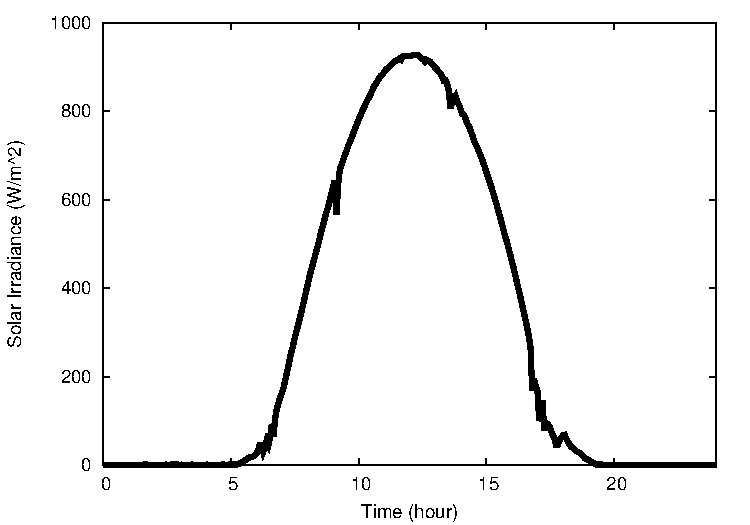
\includegraphics[width=\columnwidth]{fig/plot_1day_dec19}
		\caption{Solar irradiance during summer days.\label{fig:plot_1day_dec19}}
	\end{subfigure}%
	\begin{subfigure}[b]{0.5\textwidth}
		\centering
		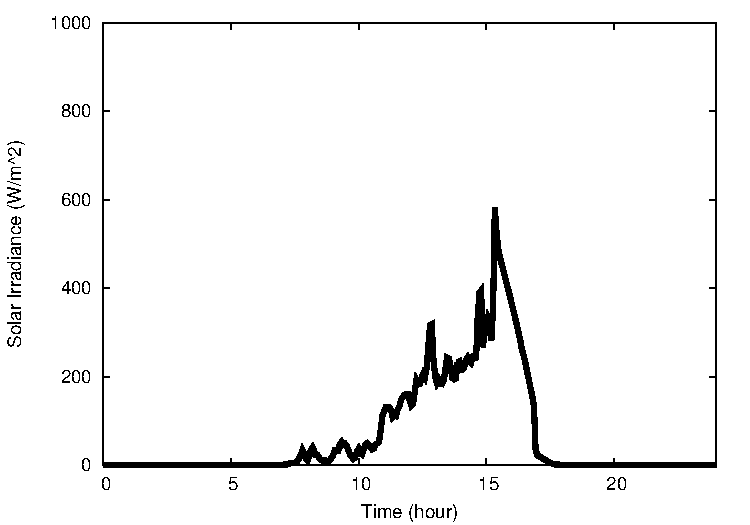
\includegraphics[width=\columnwidth]{fig/plot_1day_jun18}
		\caption{Solar irradiance during winter days.\label{fig:plot_1day_jun18}}
	\end{subfigure}%

	\begin{subfigure}[b]{0.5\textwidth}
		\centering
		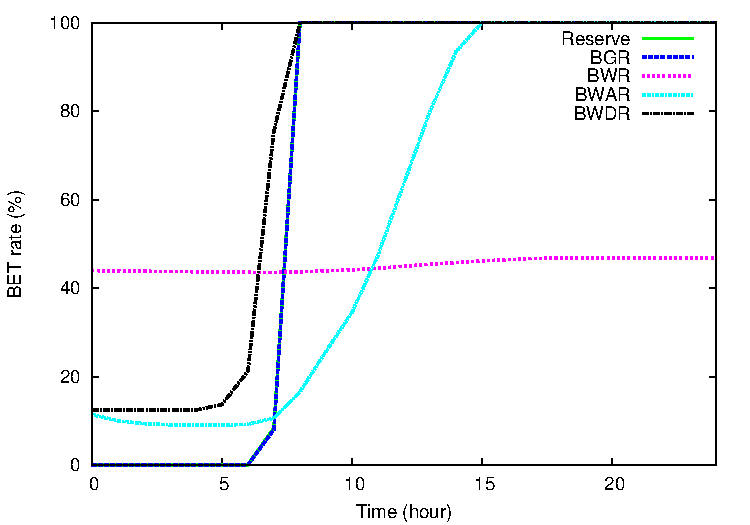
\includegraphics[width=\columnwidth]{fig/bet_rate_1h_dec19}
		\caption{BET rate during summer days.\label{fig:bet_rate_1h_dec19}}
	\end{subfigure}%
	\begin{subfigure}[b]{0.5\textwidth}
		\centering
		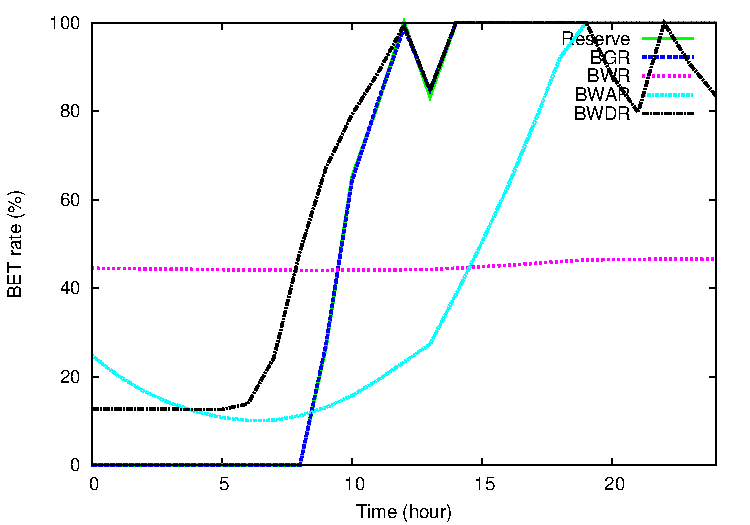
\includegraphics[width=\columnwidth]{fig/bet_rate_1h_jun18}
		\caption{BET rate during winter days.\label{fig:bet_rate_1h_jun18}}
	\end{subfigure}

    \caption{BET rate variations around the southern (summer) and northern (winter) solstices in the southern hemisphere.\label{figfour:2}}
\end{figure}


In the simulations, the hard real-time tasks fail often when the system does not perform energy scheduling.
This happens because the system runs out of energy during periods of low solar irradiation or at night.
It is also necessary to note that, on the event of a longer failure on the energy harvesting mechanism, the system would go totally down in few hours if it does not reserve energy.

Figure~\ref{figtwo:plot_1yearbet_rate_1m} shows the variations on the monthly BET rate over one year.
As can be seen, regardless of how the approaches try to reduce the impact of the lower solar irradiation in the second half of the year, all of them slightly decrease BET rate due to the diminished amount of energy coming into the system.
That variation had only been small, however, if taking into account the monthly BET rate.
Figure~\ref{figfour:1} shows the variation of the BET rate during a summer and winter months.
As can be seen, system response to irradiation is fast in all approaches except BWR.
That happens because BWR does not speculate over energy production and features a larger energy buffer.
It is also possible to note that BWAR, although presenting an operating amplitude of around 60~p.p., shows a better performance, keeping BET rate above BWR most of the time without the need for a larger energy buffer.

Figure~\ref{figfour:2} shows another characteristic of the simulated schedulers.
These figures show the BET rate around the southern (December 21st) the northern (June 20nd) solstices, which in southern Brazil should be periods of, respectively, higher and lower solar irradiation levels.
As can be seen, all approaches, except BWR and BWAR, nulled BET rate on a daily basis.

% Summarize contribution results
Summarizing the results, \bwr~(BWR) and \bwar~(BWAR) behave in much better way when compared with others.
BWR shows a remarkably stable behavior at the cost of higher demand of battery size.
BWAR, although showing a large operating amplitude, was able to execute more best-effort tasks than the others.
Also, during the whole year, the BET rate obtained through BWAR was never zero.

% Also, we analyze the impact on the network performance by comparing the
% obtained results with the data originally published by
% Okazaki~\cite{Okazaki:2011}.
% Fig.~\ref{figtwo:adzrp-avg_node_energy-adzrp-avg_node_lifetime} (above) shows a
% reduction on the average energy consumed by each node on the network while
% Fig.~\ref{figtwo:adzrp-avg_node_energy-adzrp-avg_node_lifetime} (bellow) shows
% the expected enhancement on the average battery lifetime of nodes. It is
% important to note that all nodes in the network lived for, at least, 25 days as
% expected, being that the reason why the average lifetime stayed well above it,
% around 30.

% \fig{adhop-consumption}{Average energy consumption parameters for the simulated \adhop~setup.}{width=\columnwidth}

% Besides the good results from the energy consumption perspective, we observed an
% important decrease on the overall network quality, as shown in
% Fig.~\ref{figtwo:adzrp-network_original-adzrp-network_ea} for the ``Broken
% routes'' and ``Delivery ratio'' parameters. These contrast, however, with the
% obtained results on ``Link failures'', indicating that \adhop~deals well with
% the broken routes, allowing undelivered packets to be re-routed and finally
% delivered.
% Future work on
% energy-aware scheduling, which were not focus of the present work, will rely on
% the presently proposed accounting mechanism to enable fairer scheduling of such
% tasks and handle the impact on network performance.

% \figtwo{adhop-packet_delivery}{}{adhop-data_delivery}{}{Impact on network quality: frame delivery at MAC level (top) and data delivery at network level (bottom).}


% \subsection{Characterization of application and energy models}
% 
% \fig{adhop-char-ddr_ovh}{\ldots}{width=\columnwidth}
% 
% \fig{adhop-char-mac}{\ldots}{width=\columnwidth}
% 
% \fig{adhop-char-energy}{\ldots}{width=\columnwidth}
% 
% \subsection{Simulation approach and results}
% 
% \fig{adhop-sim-plot01}{BET rate - 1month avg}{width=\columnwidth}
% 
% \fig{adhop-sim-plot02}{BET rate - 1day avg - january}{width=\columnwidth}
% 
% \fig{adhop-sim-plot03}{BET rate - 1day avg - september}{width=\columnwidth}
% 
% \fig{adhop-sim-plot04}{BET rate - 1hour avg - january 1st}{width=\columnwidth}
% 
% \fig{adhop-sim-plot05}{BET rate - 1hour avg - september 1st}{width=\columnwidth}
% 
